\section{Overview}
\begin{frame}{Partitioning of Clock Functionality}
	\begin{tikzpicture}
		\draw[white] (-2.1,.5) rectangle (9, -7);

		% individual modules
		\node[rectangle,draw=black,minimum height=.75cm,minimum width=3cm,above right] at (0,-1) {time\_buffer};
		\node[rectangle,draw=black,minimum height=.75cm,minimum width=2.1cm,above right] at (.9,-2) {time\_date};
		\node[rectangle,draw=black,minimum height=.75cm,minimum width=2.1cm,above right] at (.9,-3) {alarm};
		\node[rectangle,draw=black,minimum height=.75cm,minimum width=2.1cm,above right] at (.9,-4) {countdown};
		\node[rectangle,draw=black,minimum height=.75cm,minimum width=3cm,above right] at (5,-3) {display\_driver};
		\node[rectangle,draw=black,minimum height=.75cm,minimum width=5cm,above right] at (0,-6) {mode\_fsm};

		% clk/reset signals (enable_gen)
		\only<2> {
			\draw[white!50!black,line width=2pt,->] (-2,-6.3) -- (6,-6.3) ->  (6,-3);
			\draw[white!50!black,line width=2pt,->] (-.5,-6.3) -- (-.5,-1) -> (0,-1);
			\draw[white!50!black,line width=2pt,->] (-.5,-2) -> (.9,-2);
			\draw[white!50!black,line width=2pt,->] (-.5,-3) -> (.9,-3);
			\draw[white!50!black,line width=2pt,->] (-.5,-4) -> (.9,-4);
			\draw[white!50!black,line width=2pt,->] (-.5,-6) -> (0,-6);
			\draw[white!50!black,line width=2pt,->] (-.5,-4.5) -- (4,-4.5) -> (4,-4);
			\node[rectangle,below right] at (-2,-6.3) {enable\_gen};
		}

		% time signals
		\only<3-> {
			\draw[red!50!black,line width=2pt,->] (-1,-.625) -- (0,-.625);
			\draw[red!50!black,line width=2pt,->] (.5,-1) -- (.5,-1.5) -> (.9,-1.5);
			\draw[red!50!black,line width=2pt,->] (.5,-1) -- (.5,-2.5) -> (.9,-2.5);
			\draw[red!50!black,line width=2pt,->] (.5,-1) -- (.5,-3.5) -> (.9,-3.5);
			\node[rectangle,above right] at (-2,-.625) {dcf77\_eval};
		}

		% key status signals
		\only<4-> {
			\draw[green!50!black,line width=2pt,->] (-1,-1.75) -- (-.25,-1.75) -- (-.25,-1.75) -> (.9,-1.75);
			\draw[green!50!black,line width=2pt,->] (-1,-1.75) -- (-.25,-1.75) -- (-.25,-2.75) -> (.9,-2.75);
			\draw[green!50!black,line width=2pt,->] (-1,-1.75) -- (-.25,-1.75) -- (-.25,-3.75) -> (.9,-3.75);
			\draw[green!50!black,line width=2pt,->] (-1,-1.75) -- (-.25,-1.75) -- (-.25,-5.625) -> (0,-5.625);
			\node[rectangle,above right] at (-2,-1.75) {key\_control};
		}

		% display data signals
		\only<5-> {
			\draw[line width=2pt,->] (3,-1.625) -> (4, -1.625);
			\draw[line width=2pt,->] (3,-2.625) -> (4, -2.625);
			\draw[line width=2pt,->] (3,-3.625) -> (4, -3.625);
			\draw[line width=2pt,->] (4.5,-2.625) -> (5, -2.625);
		}

		\only<5-> {
			% status signals modules -> fsm
			% only needed for alarm since we dropped the modified signal
			% \draw[->] (3,-1.375) -- (3.4,-1.375) -> (3.4,-5.25);
			\draw[->] (3,-2.375) -- (3.3,-2.375) -> (3.3,-5.25);
			% \draw[->] (3,-3.375) -- (3.2,-3.375) -> (3.2,-5.25);

			% control signals fsm -> modules
			\draw[->] (3.8,-5.25) -- (3.8,-1.875) -> (3,-1.875);
			\draw[->] (3.7,-5.25) -- (3.7,-2.875) -> (3,-2.875);
			\draw[->] (3.6,-5.25) -- (3.6,-3.875) -> (3,-3.875);

			% mux ctl
			\draw[->] (4.25,-5.25) -> (4.25,-3.75);
		}

		\only<6-> {
			% misc outputs from modules (alarm, timer)
			\draw[blue!70!black,line width=2pt,->] (3,-2.25) -- (3.5,-2.25) -- (3.5,-.5) -> (9,-.5);
			\draw[blue!70!black,line width=2pt,->] (3,-3.25) -- (3.5,-3.25) -- (3.5,-.5) -> (9,-.5);

			% \node[rectangle,draw=black,above right] at (5,-1.75) {sw\_on<='0'};
			% \draw[blue!70!black,line width=2pt,->] (6,-1.2) -- (6,-.5) -> (9,-.5);

			% display control lines
			\draw[blue!70!black,line width=2pt,->] (8,-2.625) -> (9,-2.625);
		}

		% mux
		\draw (4,-1.25) -- (4.5, -1.75) -- (4.5,-3.5) -- (4,-4) -- cycle;
		\node[rotate=90] at (4.25,-2.625) {display\_mux};

		% top level module
		\draw[dashed,gray] (-.75,0) rectangle (8.5, -6.25);
	\end{tikzpicture}
\end{frame}

\begin{frame}{Workload Distribution}
	\begin{columns}
		\begin{column}{5cm}
			\begin{tabular}{lll}
				\rowcolor{white!80!orange}          uhrenbaustein     & Sophia    \\
				\rowcolor{white!80!orange}          mode\_alarm       & Sophia    \\
				\rowcolor{yellow!50!green!20!white} mode\_fsm         & Fabian    \\
				\rowcolor{yellow!50!green!20!white} display\_mux      & Fabian    \\
				\rowcolor{white!80!yellow}          mode\_time\_date  & Tobi      \\
				\rowcolor{white!80!yellow}          mode\_countdown   & Tobi      \\
				\rowcolor{white!80!red}             time\_buffer      & Mathias   \\
				\rowcolor{white!80!red}             display\_driver   & Mathias
			\end{tabular}
		\end{column}
		\begin{column}{6cm}
			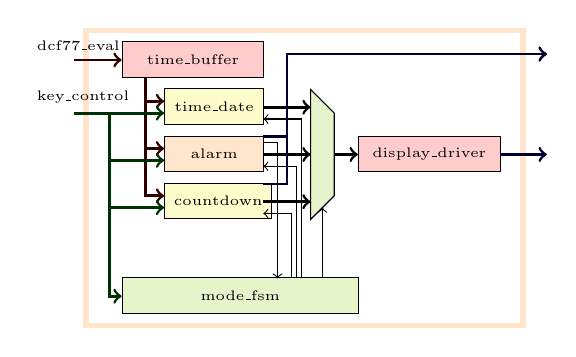
\begin{tikzpicture}[x=.6cm,y=.6cm,font=\tiny]
				% top level module
				\draw[white!80!orange,line width=2pt] (-.75,0) rectangle (8.5, -6.25);

				% individual modules
				\node[rectangle,fill=white!80!red,   draw=black,minimum height=0.45cm,minimum width=1.80cm,above right] at (0.,-1) {time\_buffer};
				\node[rectangle,fill=white!80!yellow,draw=black,minimum height=0.45cm,minimum width=1.26cm,above right] at (.9,-2) {time\_date};
				\node[rectangle,fill=white!80!orange,draw=black,minimum height=0.45cm,minimum width=1.26cm,above right] at (.9,-3) {alarm};
				\node[rectangle,fill=white!80!yellow,draw=black,minimum height=0.45cm,minimum width=1.26cm,above right] at (.9,-4) {countdown};
				\node[rectangle,fill=white!80!red,   draw=black,minimum height=0.45cm,minimum width=1.80cm,above right] at (5.,-3) {display\_driver};
				\node[rectangle,fill=yellow!50!green!20!white,draw=black,minimum height=0.45cm,minimum width=3.00cm,above right] at (0.,-6) {mode\_fsm};

				% time signals
				\draw[red!19!black,line width=1pt,->] (-1,-.625) -- (0,-.625);
				\draw[red!19!black,line width=1pt,->] (.5,-1) -- (.5,-1.5) -> (.9,-1.5);
				\draw[red!19!black,line width=1pt,->] (.5,-1) -- (.5,-2.5) -> (.9,-2.5);
				\draw[red!19!black,line width=1pt,->] (.5,-1) -- (.5,-3.5) -> (.9,-3.5);
				\node[rectangle,above right] at (-2,-.625) {dcf77\_eval};

				% key status signals
				\draw[green!19!black,line width=1pt,->] (-1,-1.75) -- (-.25,-1.75) -- (-.25,-1.75) -> (.9,-1.75);
				\draw[green!19!black,line width=1pt,->] (-1,-1.75) -- (-.25,-1.75) -- (-.25,-2.75) -> (.9,-2.75);
				\draw[green!19!black,line width=1pt,->] (-1,-1.75) -- (-.25,-1.75) -- (-.25,-3.75) -> (.9,-3.75);
				\draw[green!19!black,line width=1pt,->] (-1,-1.75) -- (-.25,-1.75) -- (-.25,-5.625) -> (0,-5.625);
				\node[rectangle,above right] at (-2,-1.75) {key\_control};

				% display data signals
				\draw[line width=1pt,->] (3,-1.625) -> (4, -1.625);
				\draw[line width=1pt,->] (3,-2.625) -> (4, -2.625);
				\draw[line width=1pt,->] (3,-3.625) -> (4, -3.625);
				\draw[line width=1pt,->] (4.5,-2.625) -> (5, -2.625);

				% status signals modules -> fsm
				% only needed for alarm since we dropped the modified signal
				% \draw[->] (3,-1.375) -- (3.4,-1.375) -> (3.4,-5.25);
				\draw[->] (3,-2.375) -- (3.3,-2.375) -> (3.3,-5.25);
				% \draw[->] (3,-3.375) -- (3.2,-3.375) -> (3.2,-5.25);

				% control signals fsm -> modules
				\draw[->] (3.8,-5.25) -- (3.8,-1.875) -> (3,-1.875);
				\draw[->] (3.7,-5.25) -- (3.7,-2.875) -> (3,-2.875);
				\draw[->] (3.6,-5.25) -- (3.6,-3.875) -> (3,-3.875);

				% mux ctl
				\draw[->] (4.25,-5.25) -> (4.25,-3.75);

				% misc outputs from modules (alarm, timer)
				\draw[blue!19!black,line width=1pt,->] (3,-2.25) -- (3.5,-2.25) -- (3.5,-.5) -> (9,-.5);
				\draw[blue!19!black,line width=1pt,->] (3,-3.25) -- (3.5,-3.25) -- (3.5,-.5) -> (9,-.5);

				% \node[rectangle,draw=black,above right] at (5,-1.75) {sw\_on<='0'};
				% \draw[blue!70!black,line width=2pt,->] (6,-1.2) -- (6,-.5) -> (9,-.5);

				% display control lines
				\draw[blue!19!black,line width=1pt,->] (8,-2.625) -> (9,-2.625);

				% mux
				\draw[fill=yellow!50!green!20!white] (4,-1.25) -- (4.5, -1.75) -- (4.5,-3.5) -- (4,-4) -- cycle;
			\end{tikzpicture}
		\end{column}
	\end{columns}
\end{frame}

\begin{frame}{Common System Integration}
	\begin{itemize}
		\item Common data format: VHDL package for all modules % already created
		\item Use git to synchronize efforts
		\item E-Mail for discussion
		\item Top level module is treated like any other module
	\end{itemize}
\end{frame}

\begin{frame}{Testing strategy}
	\begin{enumerate}
		\item person assigned to module creates individual testbench
		\item test corner cases, e.g.: \begin{itemize}
			\item correct behavior when alarm is ringing
			\item invalid DCF77 signal
			\item reset
			\item continued countdown in background
		\end{itemize}
		\item supervisor checks module and testbench after realization
		\item tests on actual hardware
	\end{enumerate}
\end{frame}

\begin{frame}{Testing strategy}
	\begin{center}
		\begin{tabular}{lll}
			\toprule
									& implement   & supervise  \\ \midrule
			uhrenbaustein     & Sophia      & Fabian     \\
			mode\_alarm       & Sophia      & Fabian     \\
			mode\_fsm         & Fabian      & Tobi       \\
			display\_mux      & Fabian      & Tobi       \\
			mode\_time\_date  & Tobi        & Mathias    \\
			mode\_countdown   & Tobi        & Mathias    \\
			display\_driver   & Mathias     & Sophia     \\
			time\_buffer      & Mathias     & Sophia     \\ \bottomrule
		\end{tabular}
	\end{center}
\end{frame}
